\section{Grundbegriffe}

\subsection{Artihmetisches Mittel}
Das arithmetische Mittel beschreibt den Mittelwert der Summe aller Elemente.

\[ \bar{x} = \frac{1}{n} \sum\limits_{i=1}^{n} x_i \]

\subsection{R-Tipps}
\subsubsection{Zahlenfolgen definieren}
Vektor für eine lineare Zahlenfolge definieren mit Intervall = 1
\begin{Schunk}
\begin{Sinput}
> x <- 1:10
> x
\end{Sinput}
\begin{Soutput}
 [1]  1  2  3  4  5  6  7  8  9 10
\end{Soutput}
\end{Schunk}
Vektor für eine Zahlenfolge mit beliebigem Intervall (z.B. 3)
\begin{Schunk}
\begin{Sinput}
> x <- seq(1,20,3)
> x
\end{Sinput}
\begin{Soutput}
[1]  1  4  7 10 13 16 19
\end{Soutput}
\end{Schunk}
Eine spezielle Zahlenfolge kann auch manuell definiert werden
\begin{Schunk}
\begin{Sinput}
> x <- c(3,2,5,8,9,10,55,1,12)
> x
\end{Sinput}
\begin{Soutput}
[1]  3  2  5  8  9 10 55  1 12
\end{Soutput}
\end{Schunk}
\subsubsection{Artihmetisches Mittel mit R berechnen}
Mit R kann das arithmetische Mittel mit der Funktion \verb!mean()! 
ermittelt werden
\begin{Schunk}
\begin{Sinput}
> x <- c(2,5,1,7,8,9)
> mean(x)
\end{Sinput}
\begin{Soutput}
[1] 5.333333
\end{Soutput}
\end{Schunk}

\subsection{Standardabweichung}
Die Standardabweichung beschreibt wie gross die mittlere Abweichung der
Beobachtungen vom arithmetischen Mittel derselben Beobachtungen ist.
\[ s_x = \sqrt{ \frac{1}{n-1} \sum\limits_{i=1}^{n} (x_i - \bar{x})^2 } \]
Bsp.: Wir nehmen eine zufällige Zahlenfolge innerhalb $(1,10)$ und
rechnen das arithmetische Mittel als auch die Standardabweichung (\verb!sd()!).
\begin{Schunk}
\begin{Sinput}
> x <- round(x=runif(n=10, min=1, max=10), digits=0)
> x
\end{Sinput}
\begin{Soutput}
 [1] 9 6 5 6 6 8 7 7 9 9
\end{Soutput}
\begin{Sinput}
> mean(x)
\end{Sinput}
\begin{Soutput}
[1] 7.2
\end{Soutput}
\begin{Sinput}
> sd(x)
\end{Sinput}
\begin{Soutput}
[1] 1.47573
\end{Soutput}
\end{Schunk}

\subsection{Quantile}
Quantile beschreiben folgenden Zusammenhang: Hat man z.B. 20 Messungen gemacht
und sortiert diese, dann beschreibt ein x\%-iges Qantil eine Punkt oder Grenze
in der Messreihe, wo x\% der Werte darunter liegen.

\[ \alpha: \text{ Prozentwert} \quad \alpha \in [0,1] \]
\[ x_1 - x_n \text{ sortiert nach grösse}  \]
\[ \alpha \cdot n \]
\[ \text{hier müssen 2 Fälle unterschieden werden: ganze Zahlen und gebrochene} \]
\[ \text{ganze Zahlen:} \quad \frac{1}{2} 
\cdot (x_{\alpha \cdot n} + x_{\alpha \cdot (n+1)}) \]
\[ \begin{array}{@{}@{}ll}
	\text{gebrochene Zahlen:} & k=\alpha \cdot n + \frac{1}{2} \\
	                          & k \text{ runden} \\
				  & \Rightarrow x_{(k)}
\end{array}\]

\begin{Schunk}
\begin{Sinput}
> x<-round(x=runif(n=20, min=1, max=20), digits=0)
> x<-sort(x)
> x
\end{Sinput}
\begin{Soutput}
 [1]  3  4  6  6  7  7 10 11 11 12 12 12 16 16 16 18 18 18 20 20
\end{Soutput}
\begin{Sinput}
> quantile(x, prob=0.2)
\end{Sinput}
\begin{Soutput}
20% 
6.8 
\end{Soutput}
\begin{Sinput}
> quantile(x, prob=0.2, type=1)
\end{Sinput}
\begin{Soutput}
20% 
  6 
\end{Soutput}
\begin{Sinput}
> quantile(x, prob=0.2, type=2)
\end{Sinput}
\begin{Soutput}
20% 
6.5 
\end{Soutput}
\end{Schunk}
Im obigen Beispiel wird mit R das 20\%-Quantil bestimmt. Hier ist aber 
Vorsicht geboten, denn R hat 9 verschiedene \verb!type! für die Funktion
\verb!quantile()! (default-Wert ist 7). Für uns aus dem 
Stochastik-Modul ist der \verb!type=2! 
der einzig richtige Wert!

\subsection{Median}
Der Median ist ein Spezialfall der Quantile, nämlich ist dies jenes Quantil,
welches die 50\%-Marke beschreibt.

Bsp.: Wir haben 5 Personen, und messen deren Höhe. Danach sortieren wir die
Ergebnisse. Der Median ist nun jene Person in der Mitte (unabhängig von seiner
genauen Höhe!). Interssant oder eben speziell am Median ist,
dass es immer die selbe Person bleibt auch wenn die kleineren und grösseren
noch grösser und noch kleiner werden. Dies bedeutet, dass der Median 
unempfindlich gegenüber sog. Ausreissern ist (denke an Durchschnittsvermögen
in einem Land mit vielen Armen und wenigen aber extrem Reichen).
\begin{Schunk}
\begin{Sinput}
> x <- c(1.6, 1.7, 1.75, 1.87, 1.94)
> median(x)
\end{Sinput}
\begin{Soutput}
[1] 1.75
\end{Soutput}
\begin{Sinput}
> x <- c(1.2, 1.4, 1.75, 1.99, 2.14)
> median(x)
\end{Sinput}
\begin{Soutput}
[1] 1.75
\end{Soutput}
\end{Schunk}

\subsection{Varianz}
Die Varianz beschreibt die quadratische Abweichung von Daten von ihrem 
arithmetischen Mittelwert. Sie ist das Quadrat der Standardabweichung. 
\[ {s_x}^2 = \frac{1}{n-1} \sum\limits_{i=1}^{n} (x_i - \bar{x})^2 \]
\begin{Schunk}
\begin{Sinput}
> x=runif(n=10)
> y=runif(n=10)
> var(x)
\end{Sinput}
\begin{Soutput}
[1] 0.08093076
\end{Soutput}
\end{Schunk}

\subsection{Kovarianz}
Die Kovarianz beschreibt, wie stark die Abweichungen von zwei Vektoren von 
ihren jeweiligen arithmetischen Mittelwerten korrelieren. Die Kovarianz 
eines Vektors mit sich selbst entspricht der Varianz des Vektors. 
\[ s_{xy} 
= \frac{1}{n-1} \sum\limits_{i=1}^{n} (x_i - \bar{x}) (y_i - \bar{y}) \]
\begin{Schunk}
\begin{Sinput}
> cov(x,y)
\end{Sinput}
\begin{Soutput}
[1] 0.04662218
\end{Soutput}
\end{Schunk}

\subsection{Korrelationskoeffizient}
Der Korrelationskoeffizient beschreibt die Linearität von zwei Vektoren 
zueinander. Der Wertebereich des Korrelationskoeffizienten ist $[-1, 1]$. 
\[ r = \frac{s_{xy}}{s_x \cdot s_y} 
= \frac{\sum\limits_{i=1}^{n} (x_i - \bar{x}) (y_i - \bar{y})}
{\sqrt{\sum\limits_{i=1}^{n} (x_i - \bar{x})^2  \cdot 
\sum\limits_{i=1}^{n} (y_i - \bar{y})^2 }} \]
\begin{Schunk}
\begin{Sinput}
> cor(x,y)
\end{Sinput}
\begin{Soutput}
[1] 0.498205
\end{Soutput}
\end{Schunk}

\section{Diskrete Verteilungen}

\subsection{Hypergeometrische Verteilung}
Die Hypergeometrische Verteilung beschreibt die Wahrscheinlichkeit beim 
Ziehen ohne zurücklegen. Im folgenden Beispiel mit farbigen Kugeln. 
\[ X \sim Hyp(n, r, s) \]
\begin{tabular}{@{}ll}
  $n$: & Anzahl Ziehungen \\
  $r$: & Anzahl rote Kugeln in der Urne (positive Ergebnisse) \\
  $s$: & Anzahl schwarze Kugeln in der Urne (negative Ergebnisse) \\
  $N$: & Anzahl Kugeln in der Urne ($N = r + s$)
\end{tabular}
\[ P(X=k) 
= \frac{\left( \begin{array}{c}r\\k\end{array} \right) \cdot 
\left( \begin{array}{c}s\\n-k\end{array} \right)}
{\left( \begin{array}{c}r+s\\n\end{array} \right)} 
= \frac{\left( \begin{array}{c}r\\k\end{array} \right) \cdot 
\left( \begin{array}{c}N-r\\n-k\end{array} \right)}
{\left( \begin{array}{c}N\\n\end{array} \right)} \]
\begin{Schunk}
\begin{Sinput}
> k=6;
> n=6;
> r=6;
> s=36;
> dhyper(x=k,m=r,n=s,k=n)
\end{Sinput}
\begin{Soutput}
[1] 1.906292e-07
\end{Soutput}
\end{Schunk}
\subsubsection{Kumulative Verteilungsfunktion}
\begin{Schunk}
\begin{Sinput}
> q=1;
> phyper(q=q,m=r,n=s,k=n)
\end{Sinput}
\begin{Soutput}
[1] 0.8025001
\end{Soutput}
\end{Schunk}

\subsection{Binomialverteilung}
Die Binomialverteilung kann bei Ereignissen eingesetzt werden, die zwei 
mögliche Ergebnisse zeigen können. Sie ist ein Grenzfall der 
Hypergeometrischen Verteilung. 
\footnote{Beispiele für Ereignisse mit zwei möglichen Ergebnissen: 
  \begin{itemize} 
    \item Münzwurf $\Rightarrow$ Kopf $\leftrightarrow$ Zahl
    \item Würfeln $\Rightarrow$ Sechser $\leftrightarrow$ kein Sechser
  \end{itemize}}
Die Wahrscheinlichkeit ist dann wie folgt gegeben: 
\[ P(X=x) = 
\left( \begin{array}{c}n\\x\end{array} \right) \cdot p^x \cdot (1-p)^{n-x} 
= \frac{n!}{x! (n-x)!} \cdot p^x \cdot (1-p)^{n-x} \]
\begin{tabular}{@{}ll}
  $n$: & Anzahl Versuche \\
  $x$: & Anzahl Versuche mit positivem Ergebnis \\
  $p$: & Wahrscheinlichkeit für ein positives Ergebnis jedem einzelnen Versuch
\end{tabular} 
\begin{Schunk}
\begin{Sinput}
> n=5;
> x=3;
> p=0.2;
> dbinom(x=x,size=n,prob=p)
\end{Sinput}
\begin{Soutput}
[1] 0.0512
\end{Soutput}
\end{Schunk}
\subsubsection{Kumulative Verteilungsfunktion}
\begin{Schunk}
\begin{Sinput}
> q=3;
> pbinom(q=q,size=n,prob=p)
\end{Sinput}
\begin{Soutput}
[1] 0.99328
\end{Soutput}
\end{Schunk}

\subsection{Poissonverteilung}
Die Poissonverteilung wird bei Ereignissen verwendet, deren maximale Anzahl 
nicht begrenzt ist. Sie ist ein Grenzfall der Binomialverteilung. 
\[ P(X=x) = \exp(-\lambda) \cdot \frac{\lambda^x}{x!} \]
\begin{tabular}{@{}ll}
  $x$: & Anzahl Versuche mit positivem Ergebnis \\
  $\lambda$: & Erwartungswert
\end{tabular} 
\begin{Schunk}
\begin{Sinput}
> lambda=2;
> x=3;
> dpois(x=x,lambda=lambda)
\end{Sinput}
\begin{Soutput}
[1] 0.180447
\end{Soutput}
\end{Schunk}

\subsubsection{Kumulative Verteilungsfunktion}
\begin{Schunk}
\begin{Sinput}
> q=3;
> ppois(q=q,lambda=lambda)
\end{Sinput}
\begin{Soutput}
[1] 0.8571235
\end{Soutput}
\end{Schunk}

\section{Stetige Verteilungen}

\subsection{Uniform}
\begin{Schunk}
\begin{Sinput}
> x=3;
> min=2;
> max=5;
> dunif(x=x,min=min,max=max)
\end{Sinput}
\begin{Soutput}
[1] 0.3333333
\end{Soutput}
\begin{Sinput}
> range=seq(from=0,to=10,by=0.001);
> plot(range,dunif(x=range,min=min,max=max),type='l')
\end{Sinput}
\end{Schunk}
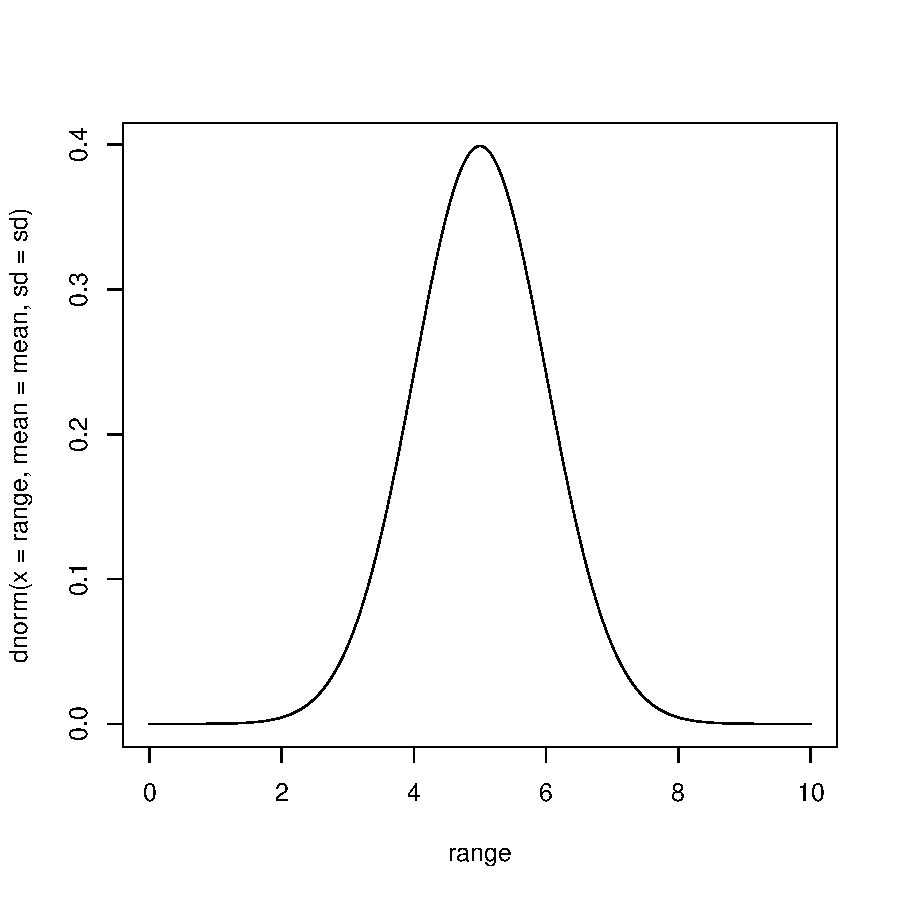
\includegraphics{definitionen-017}

\subsubsection{Kumulative Verteilungsfunktion}
\begin{Schunk}
\begin{Sinput}
> q=3;
> punif(q=q,min=min,max=max)
\end{Sinput}
\begin{Soutput}
[1] 0.3333333
\end{Soutput}
\end{Schunk}

\subsection{Normalverteilung}
\begin{Schunk}
\begin{Sinput}
> x=7;
> mean=5;
> sd=1;
> dnorm(x=x,mean=mean,sd=sd)
\end{Sinput}
\begin{Soutput}
[1] 0.05399097
\end{Soutput}
\begin{Sinput}
> range=seq(from=0,to=10,by=0.001);
> plot(range,dnorm(x=range,mean=mean,sd=sd),type='l')
\end{Sinput}
\end{Schunk}
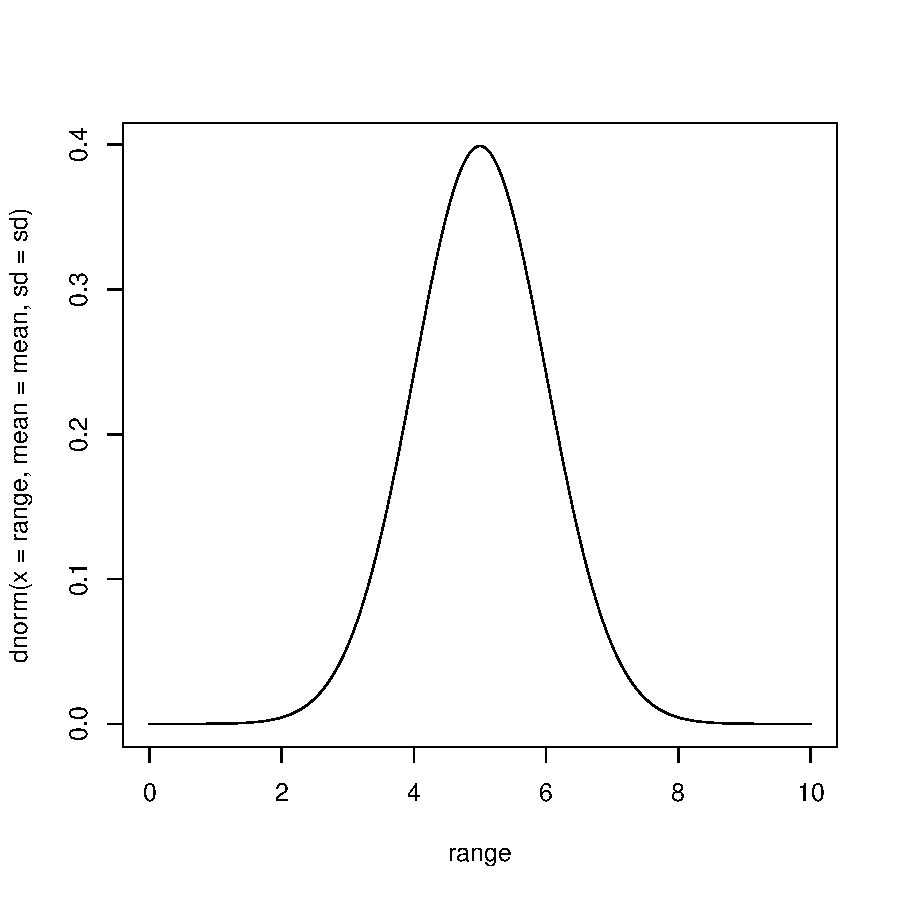
\includegraphics{definitionen-019}

\subsubsection{Kumulative Verteilungsfunktion}
\begin{Schunk}
\begin{Sinput}
> q=7;
> pnorm(q=q,mean=mean,sd=sd)
\end{Sinput}
\begin{Soutput}
[1] 0.9772499
\end{Soutput}
\end{Schunk}

\subsection{Exponentialverteilung}
\begin{Schunk}
\begin{Sinput}
> x=3;
> lambda=2;
> dexp(x=x,rate=lambda)
\end{Sinput}
\begin{Soutput}
[1] 0.004957504
\end{Soutput}
\begin{Sinput}
> range=seq(from=0,to=10,by=0.001);
> plot(range,dexp(x=range,rate=lambda),type='l')
\end{Sinput}
\end{Schunk}
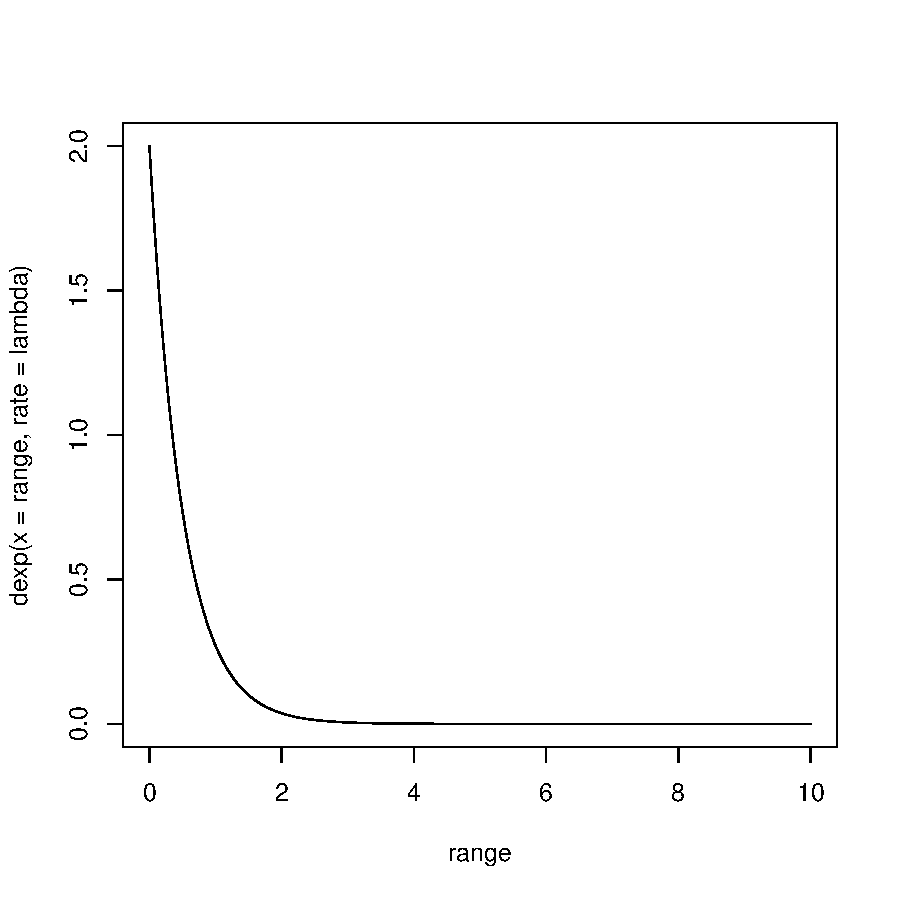
\includegraphics{definitionen-021}

\subsubsection{Kumulative Verteilungsfunktion}
\begin{Schunk}
\begin{Sinput}
> q=3;
> pexp(q=q,rate=lambda)
\end{Sinput}
\begin{Soutput}
[1] 0.9975212
\end{Soutput}
\end{Schunk}

\section{Statistischer Test}
Beim statistischen Test wird überprüft, ob eine statistische Verteilung zu 
ermittelten Daten passt. Dieser Test besteht aus 6 Schritten. 

\subsection{allgemeiner Ablauf}
\begin{enumerate}
  \item Modell
        Verteilung bestimmen
  \item Nullhypothese
        Nullhypothese und Alternativhypotese aufstellen
  \item Teststatistik
        Teststatistik aus Modell und Nullhypothese erstellen
  \item Signifikanzniveau
        Signifikanzniveau festlegen
  \item Verwerfungsbereich
        Aus Teststatistik und Signifikanzniveau Verwerfungsbereich berechnen
  \item Testentscheid
        Messwert mit Verwerfungsbereich vergleichen
\end{enumerate}
